%EKG-7 Realisierung/Display und UI

\subsection{Display und Benutzeroberfläche}

Dieses Unterkapitel behandelt die Auswahl des Displays und die Programmierung der Benutzeroberfläche.

\subsubsection{Auswahl des Displays}
Gesteuert wird das EKG-Gerät durch das NX4024T032. Dabei handelt es sich um ein Touch-Display der Firma Nextion. Das Display ist 3,2 Zoll groß und weist eine Auflösung von 400x240 Pixel auf. Betrieben wird das Display mit 5 V und verbraucht bei maximaler Helligkeit 85mA. Verbunden wird das Display via UART mit einer Baudrate von 115200 bps.

\subsubsection{Programmierung der Benutzeroberfläche}
Der erste Schritt der Displayprogrammierung ist die Initialisierung. In diesem Schritt wird die Baudrate von 115200 bps und die „Tap-to-wake“ Funktion integriert. Das Display schaltet sich je nachdem, auf welcher Seite man sich befindet, nach 30 bis 180 Sekunden in den Sleep-Mode. Durch einmaliges antippen auf das Display wird es wieder aufgeweckt.

Der Nextion-Editor verfügt über ein weites Spektrum von Tools. Für das Projekt wurden im wesentlichen folgende Tools verwendet:
\begin{enumerate}
    \item Text: Für die Beschreibung der Funktionen und Anleitung
    \item Number: Variablen für den Timer, Ladestand und Herzfrequenz
    \item Button: Zum Seitenwechsel und senden der Interrupts an die MCU
    \item Waveform: Für den EKG-Kurvenverlauf
    \item Slider: Einstellung der Helligkeit
    \item Interne Timer: Befehle, die regelmäßig ausgeführt werden
\end{enumerate}

Aufgebaut ist das UI aus verschiedenen Seiten. Nach dem Einschalten des EKG-Gerätes gelangt man auf die Startseite (siehe Abbildung 8). Hier ist in der oberen rechten Ecke die Peripherie zu sehen. Der Akkustand wird in Prozent angegeben und die Verbindung zur SD-Karte und zum Bluetooth-Modul überprüft. Bei einem blauen Symbol besteht eine Verbindung und bei einem grauen Symbol ist das Modul getrennt bzw. nicht verbunden. Alle Icons, die auf dem Display vorzufinden sind, wurden aus Vorlagen an das gesamte Theme angepasst. Dabei wurde die Software GIMP verwendet.
\begin{figure} [!h]
	\centering
	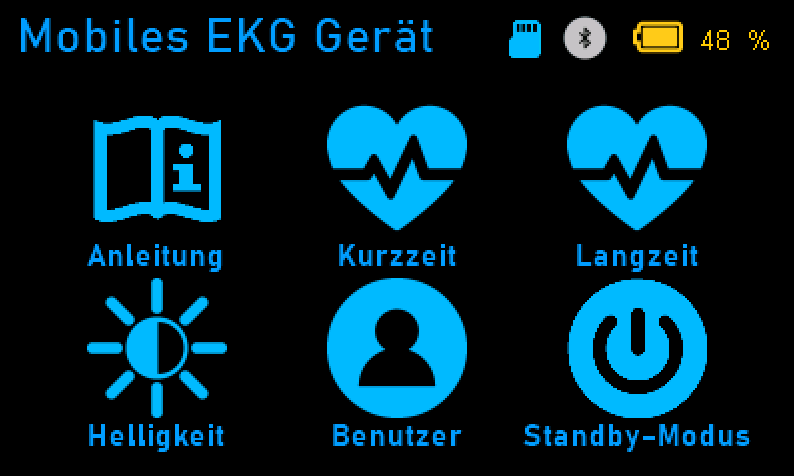
\includegraphics[width=10cm] {ECG_Homescreen.png}
	\caption{Startseite des EKG-Gerätes}
\end{figure}

Die sechs Symbole in der Mitte des Displays sind Buttons, mit denen zwischen den Seiten gewechselt wird. In der Anleitung werden allgemeine Einstellungen erklärt, wie die Elektroden am Patienten anzubringen sind und welche Funktionen ein Kurzzeit- und Langzeit-EKG bietet. Beim Kurzzeit-EKG erfolgt eine zweiminütige Aufzeichnung, welche in Echtzeit auf dem Display nachverfolgt werden kann. Beim Langzeit-EKG erfolgt die EKG-Aufnahme für 24 Stunden. Die Helligkeit des Displays kann mithilfe eines Schiebereglers eingestellt werden. Optional kann ein Benutzer ausgewählt werden. Dieser Benutzer erscheint dann auf der erstellten CSV Datei der SD-Karte. Der Standby-Modus: Versetzt das Display beim Drücken in den Sleep-Modus.

Während der Nutzung des EKG-Gerätes sind diverse Sicherheitsabfragen auf dem Display vorzufinden, wenn:
\begin{enumerate}
    \item bereits eine Aufnahme läuft und eine Andere gestartet wird.
    \item eine Aufnahme mit dem Stopp-Befehl abgebrochen wird.
    \item die SD-Karte entfernt wird oder beim Anschaltvorgang fehlt.
    \item der Ladestand des Akkus bei einer Langzeit-Aufnahme kleiner als 80 \% ist.
    \item Verdacht auf Bradykardie oder Tachykardie besteht.
\end{enumerate}

Die Herzfrequenz wird während einer Kurzzeit-Aufnahme kontinuierlich berechnet. Da es sich bei diesem Projekt um ein Ruhe-EKG handelt, sollte die Herzfrequenz im Ruhebereich liegen. Im Fall von Bradykardie oder Tachykardie wird der Patient auf dem Display visuell gewarnt.

